\documentclass[aspectratio=169, 11pt]{beamer}

\usetheme{default}
\usecolortheme{default}
\setbeamertemplate{navigation symbols}{}
\setbeamertemplate{footline}[frame number]
\setbeamerfont{frametitle}{size=\Large, series=\bfseries}
\setbeamercolor{frametitle}{fg=blue!50!black}

\usepackage{amsmath}
\usepackage{booktabs}
\usepackage{graphicx}
\usepackage[backend=biber, style=numeric, url=false, doi=false, isbn=false, eprint=false]{biblatex}
\addbibresource{../references.bib}
\graphicspath{{../figures/}}
\newcommand{\nRaw}{53{,}488}
\newcommand{\rawStart}{01 January 2016 00:00}
\newcommand{\rawEnd}{06 February 2022 17:00}
\newcommand{\nMissingHours}{2}
\newcommand{\missingHours}{30 October 2016 01:00 and 31 October 2021 01:00}
\newcommand{\priceMatch}{100.0}
\newcommand{\consRatioMin}{2.000}
\newcommand{\consRatioMax}{2.000}
\newcommand{\corConsBuy}{0.972}
\newcommand{\meanCons}{4{,}141}
\newcommand{\meanBuy}{4{,}088}
\newcommand{\meanNpCons}{8{,}282}
\newcommand{\nKnots}{318}
\newcommand{\knotWeekday}{Friday}
\newcommand{\nAfterLastKnot}{63}
\newcommand{\nNoReservoir}{71}
\newcommand{\nMissingPrice}{2{,}562}
\newcommand{\nMissingPriceAll}{2{,}562}
\newcommand{\missPriceTopYear}{2018}
\newcommand{\missPriceTopN}{858}
\newcommand{\missPriceRuns}{1{,}509}
\newcommand{\missPriceMaxRun}{13}
\newcommand{\missPriceRunsShort}{82}
\newcommand{\nClean}{50{,}855}
\newcommand{\pctRemoved}{4.9}
\newcommand{\cleanStart}{04 January 2016}
\newcommand{\cleanEnd}{06 February 2022}
\newcommand{\nNeg}{10}
\newcommand{\nZero}{1}
\newcommand{\nNonPos}{11}
\newcommand{\minPrice}{\ensuremath{-}1.97}
\newcommand{\maxPrice}{600.16}
\newcommand{\maxPriceTime}{21 December 2021 at 17:00}
\newcommand{\nAboveTwoHundred}{246}
\newcommand{\nAboveTwoHundredPct}{0.5}
\newcommand{\nYearTwentyTwo}{883}
\newcommand{\meanPrice}{39.0}
\newcommand{\medianPrice}{32.4}
\newcommand{\sdPrice}{32.5}
\newcommand{\meanConsClean}{4{,}143}
\newcommand{\sdCons}{1{,}344}
\newcommand{\minConsClean}{1{,}636}
\newcommand{\maxConsClean}{8{,}133}
\newcommand{\minRes}{7.1}
\newcommand{\maxRes}{99.8}
\newcommand{\meanPriceYI}{26.5}
\newcommand{\meanPriceYII}{29.2}
\newcommand{\meanPriceYIII}{44.1}
\newcommand{\meanPriceYIV}{39.3}
\newcommand{\meanPriceYV}{9.1}
\newcommand{\meanPriceYVI}{74.9}
\newcommand{\meanPriceYVII}{138.8}
\newcommand{\meanResYI}{60.2}
\newcommand{\meanResYII}{58.4}
\newcommand{\meanResYIII}{59.7}
\newcommand{\meanResYIV}{63.3}
\newcommand{\meanResYV}{68.9}
\newcommand{\meanResYVI}{59.6}
\newcommand{\meanResYVII}{43.5}
\newcommand{\hourMinMean}{34.2}
\newcommand{\hourMinAt}{3}
\newcommand{\hourMaxMean}{43.2}
\newcommand{\hourMaxAt}{8}
\newcommand{\monthMinMean}{28.3}
\newcommand{\monthMinAt}{June}
\newcommand{\monthMaxMean}{59.5}
\newcommand{\monthMaxAt}{December}
\newcommand{\corPriceCons}{0.21}
\newcommand{\corPriceRes}{\ensuremath{-}0.02}
\newcommand{\corConsRes}{\ensuremath{-}0.31}
\newcommand{\corYearRes}{0.03}
\newcommand{\corYearCons}{0.00}
\newcommand{\corYearPrice}{0.37}
\newcommand{\nScatterSample}{10{,}000}
\newcommand{\nAboveYlim}{109}
\newcommand{\nPar}{49}
\newcommand{\rTwo}{0.667}
\newcommand{\rTwoPct}{66.7}
\newcommand{\rse}{18.75}
\newcommand{\dfRes}{50{,}806}
\newcommand{\nullDev}{53.71}
\newcommand{\resDev}{17.87}
\newcommand{\aicFull}{442{,}519}
\newcommand{\bicFull}{442{,}961}
\newcommand{\bIntercept}{52.27}
\newcommand{\seIntercept}{1.27}
\newcommand{\ciLIntercept}{49.78}
\newcommand{\ciUIntercept}{54.77}
\newcommand{\bHourNight}{\ensuremath{-}2.04}
\newcommand{\seHourNight}{0.59}
\newcommand{\ciLHourNight}{\ensuremath{-}3.19}
\newcommand{\ciUHourNight}{\ensuremath{-}0.88}
\newcommand{\bHourMorning}{5.25}
\newcommand{\seHourMorning}{0.59}
\newcommand{\ciLHourMorning}{4.09}
\newcommand{\ciUHourMorning}{6.42}
\newcommand{\bHourEvening}{4.37}
\newcommand{\seHourEvening}{0.59}
\newcommand{\ciLHourEvening}{3.21}
\newcommand{\ciUHourEvening}{5.53}
\newcommand{\bApr}{\ensuremath{-}31.99}
\newcommand{\seApr}{0.69}
\newcommand{\ciLApr}{\ensuremath{-}33.35}
\newcommand{\ciUApr}{\ensuremath{-}30.64}
\newcommand{\bJul}{18.65}
\newcommand{\seJul}{0.75}
\newcommand{\ciLJul}{17.17}
\newcommand{\ciUJul}{20.12}
\newcommand{\bDec}{33.41}
\newcommand{\seDec}{0.45}
\newcommand{\ciLDec}{32.53}
\newcommand{\ciUDec}{34.28}
\newcommand{\bSat}{\ensuremath{-}3.03}
\newcommand{\seSat}{0.32}
\newcommand{\ciLSat}{\ensuremath{-}3.65}
\newcommand{\ciUSat}{\ensuremath{-}2.41}
\newcommand{\bSun}{\ensuremath{-}4.20}
\newcommand{\seSun}{0.32}
\newcommand{\ciLSun}{\ensuremath{-}4.83}
\newcommand{\ciUSun}{\ensuremath{-}3.57}
\newcommand{\bYeighteen}{18.11}
\newcommand{\seYeighteen}{0.29}
\newcommand{\ciLYeighteen}{17.53}
\newcommand{\ciUYeighteen}{18.69}
\newcommand{\bYtwenty}{\ensuremath{-}9.87}
\newcommand{\seYtwenty}{0.31}
\newcommand{\ciLYtwenty}{\ensuremath{-}10.47}
\newcommand{\ciUYtwenty}{\ensuremath{-}9.27}
\newcommand{\bYtwentyone}{48.97}
\newcommand{\seYtwentyone}{0.29}
\newcommand{\ciLYtwentyone}{48.41}
\newcommand{\ciUYtwentyone}{49.54}
\newcommand{\bYtwentytwo}{108.94}
\newcommand{\seYtwentytwo}{0.72}
\newcommand{\ciLYtwentytwo}{107.53}
\newcommand{\ciUYtwentytwo}{110.35}
\newcommand{\bCons}{2.08}
\newcommand{\seCons}{0.17}
\newcommand{\ciLCons}{1.74}
\newcommand{\ciUCons}{2.42}
\newcommand{\bRes}{\ensuremath{-}0.71}
\newcommand{\seRes}{0.011}
\newcommand{\ciLRes}{\ensuremath{-}0.73}
\newcommand{\ciURes}{\ensuremath{-}0.69}
\newcommand{\hNight}{03}
\newcommand{\hMorning}{08}
\newcommand{\hEvening}{17}
\newcommand{\bResTen}{\ensuremath{-}7.1}
\newcommand{\bResTenAbs}{7.1}
\newcommand{\ciLResTen}{\ensuremath{-}7.3}
\newcommand{\ciUResTen}{\ensuremath{-}6.9}
\newcommand{\bConsOne}{2.1}
\newcommand{\bConsSD}{2.8}
\newcommand{\bResSD}{\ensuremath{-}18.8}
\newcommand{\bResSDAbs}{18.8}
\newcommand{\sdConsGWh}{1.34}
\newcommand{\sdResPct}{26.4}
\newcommand{\peakDiff}{7.3}
\newcommand{\wdayPMax}{0.580}
\newcommand{\nHourNotSig}{5}
\newcommand{\dRtwoHour}{0.27}
\newcommand{\dRtwoMonth}{7.25}
\newcommand{\dRtwoWeekday}{0.20}
\newcommand{\dRtwoYear}{44.19}
\newcommand{\dRtwoConsumption}{0.10}
\newcommand{\dRtwoReservoir}{2.86}
\newcommand{\dAICHour}{370}
\newcommand{\dAICMonth}{10{,}003}
\newcommand{\dAICWeekday}{295}
\newcommand{\dAICYear}{42{,}966}
\newcommand{\dAICConsumption}{144}
\newcommand{\dAICReservoir}{4{,}192}
\newcommand{\FHour}{18.1}
\newcommand{\FMonth}{1{,}006.4}
\newcommand{\FWeekday}{51.3}
\newcommand{\FYear}{11{,}247.2}
\newcommand{\FConsumption}{145.6}
\newcommand{\FReservoir}{4{,}367.6}
\newcommand{\minF}{18.1}
\newcommand{\rTwoCal}{0.637}
\newcommand{\rTwoCalPct}{63.7}
\newcommand{\rTwoYearOnly}{55.9}
\newcommand{\vifHour}{1.7}
\newcommand{\vifMonth}{79.8}
\newcommand{\vifWeekday}{1.1}
\newcommand{\vifYear}{1.5}
\newcommand{\vifConsumption}{7.8}
\newcommand{\vifReservoir}{11.7}
\newcommand{\vifadjHour}{1.01}
\newcommand{\vifadjMonth}{1.22}
\newcommand{\vifadjWeekday}{1.01}
\newcommand{\vifadjYear}{1.03}
\newcommand{\vifadjConsumption}{2.79}
\newcommand{\vifadjReservoir}{3.42}
\newcommand{\auxResMonth}{89.4}
\newcommand{\auxResYear}{2.6}
\newcommand{\auxResAll}{91.4}
\newcommand{\auxConsMonth}{76.4}
\newcommand{\auxConsYear}{1.6}
\newcommand{\auxConsAll}{87.1}
\newcommand{\pctOutThree}{1.08}
\newcommand{\pctOutThreeNormal}{0.27}
\newcommand{\nOutThree}{551}
\newcommand{\maxResid}{489.1}
\newcommand{\skewResid}{6.09}
\newcommand{\kurtResid}{94.6}
\newcommand{\resSDYI}{10.7}
\newcommand{\resSDYII}{8.7}
\newcommand{\resSDYIII}{11.6}
\newcommand{\resSDYIV}{12.3}
\newcommand{\resSDYV}{9.1}
\newcommand{\resSDYVI}{38.3}
\newcommand{\resSDYVII}{25.5}
\newcommand{\pctLagOneIsHour}{97.0}
\newcommand{\acfOne}{0.961}
\newcommand{\acfTwentyfour}{0.743}
\newcommand{\acfWeek}{0.509}
\newcommand{\pacfOne}{0.961}
\newcommand{\pacfTwo}{\ensuremath{-}0.191}
\newcommand{\pacfTwentyfour}{\ensuremath{-}0.044}
\newcommand{\dw}{0.078}
\newcommand{\dwP}{\ensuremath{<0.001}}
\newcommand{\dwRho}{0.961}
\newcommand{\hacRatioMin}{2.2}
\newcommand{\hacRatioMax}{15.3}
\newcommand{\seHacCons}{1.50}
\newcommand{\pHacCons}{0.164}
\newcommand{\ciLHacCons}{\ensuremath{-}0.85}
\newcommand{\ciUHacCons}{5.01}
\newcommand{\seHacRes}{0.152}
\newcommand{\pHacRes}{\ensuremath{<0.001}}
\newcommand{\ciLHacResTen}{\ensuremath{-}10.1}
\newcommand{\ciUHacResTen}{\ensuremath{-}4.1}
\newcommand{\seHacMorning}{1.35}
\newcommand{\pHacMorning}{\ensuremath{<0.001}}
\newcommand{\seHacJul}{6.76}
\newcommand{\seHacYtwentyone}{4.38}
\newcommand{\pHacSun}{\ensuremath{<0.001}}
\newcommand{\binResMax}{10.2}
\newcommand{\binResMin}{\ensuremath{-}4.7}
\newcommand{\binConsMax}{2.4}
\newcommand{\binConsMin}{\ensuremath{-}1.8}
\newcommand{\kIndexCons}{1.00}
\newcommand{\kIndexRes}{0.44}
\newcommand{\binTopLo}{47}
\newcommand{\binTopHi}{60}
\newcommand{\binTopPctDec}{9}
\newcommand{\binTopResWithDec}{10.2}
\newcommand{\binTopResNoDec}{2.5}
\newcommand{\edfCons}{8.9}
\newcommand{\edfRes}{8.9}
\newcommand{\gamDevDiff}{1.75}
\newcommand{\gamF}{343.2}
\newcommand{\gamFp}{\ensuremath{<0.001}}
\newcommand{\gamDf}{16.1}
\newcommand{\rTwoGam}{0.700}
\newcommand{\rTwoGamPct}{70.0}
\newcommand{\rseGam}{17.81}
\newcommand{\aicGam}{437{,}297}
\newcommand{\bicGam}{437{,}880}
\newcommand{\dAICGam}{5{,}222}
\newcommand{\dBICGam}{5{,}081}
\newcommand{\kMax}{9}
\newcommand{\gamResBumpAt}{53}
\newcommand{\gamResTenToForty}{21.9}
\newcommand{\gamResBumpToNinetyFive}{58.1}
\newcommand{\gamResFortyToBump}{7.1}
\newcommand{\gamConsTwoToSeven}{1.7}
\newcommand{\gamConsSevenToEight}{42.9}
\newcommand{\nConsAboveSeven}{992}
\newcommand{\pctConsAboveSeven}{2.0}
\newcommand{\pctConsAboveSevenCrisis}{1}
\newcommand{\meanPriceConsAboveSeven}{62.0}
\newcommand{\nCrisis}{3{,}811}
\newcommand{\meanPriceCrisis}{125.5}
\newcommand{\meanResCrisis}{66.2}
\newcommand{\resDecTwentyOne}{71.0}
\newcommand{\resvDecTwentyOne}{60.8}
\newcommand{\priceDecTwentyOne}{174.3}
\newcommand{\pctOutThreeCrisis}{80}
\newcommand{\edfGamTotal}{64.8}
\newcommand{\aicCal}{446{,}897}
\newcommand{\bicCal}{447{,}321}

\newcommand{\eur}{EUR/MWh}
\newcommand{\bs}[1]{\boldsymbol{#1}}

\title{What drives the hourly electricity price in NO1?}
\subtitle{A Gaussian GLM with calendar effects, consumption and reservoir level}
\author{Sondre Erdi Solbakken}
\institute{STAT201 project}
\date{October 2026}

\begin{document}

%------------------------------------------------------------
\begin{frame}
\titlepage
\end{frame}

%------------------------------------------------------------
\begin{frame}{Research question}
\begin{columns}[T]
\begin{column}{0.5\textwidth}
\begin{itemize}
\item Day-ahead price in NO1 (Oslo region), one price per hour
\item NO1: much consumption, power mostly from hydro
\item[]
\item \textbf{Question:} how much of the hourly price is explained by hour, month, weekday, year, consumption and reservoir level? Which matter most?
\item[]
\item Hypothesis: demand matters, reservoir level even more
\end{itemize}
\end{column}
\begin{column}{0.5\textwidth}
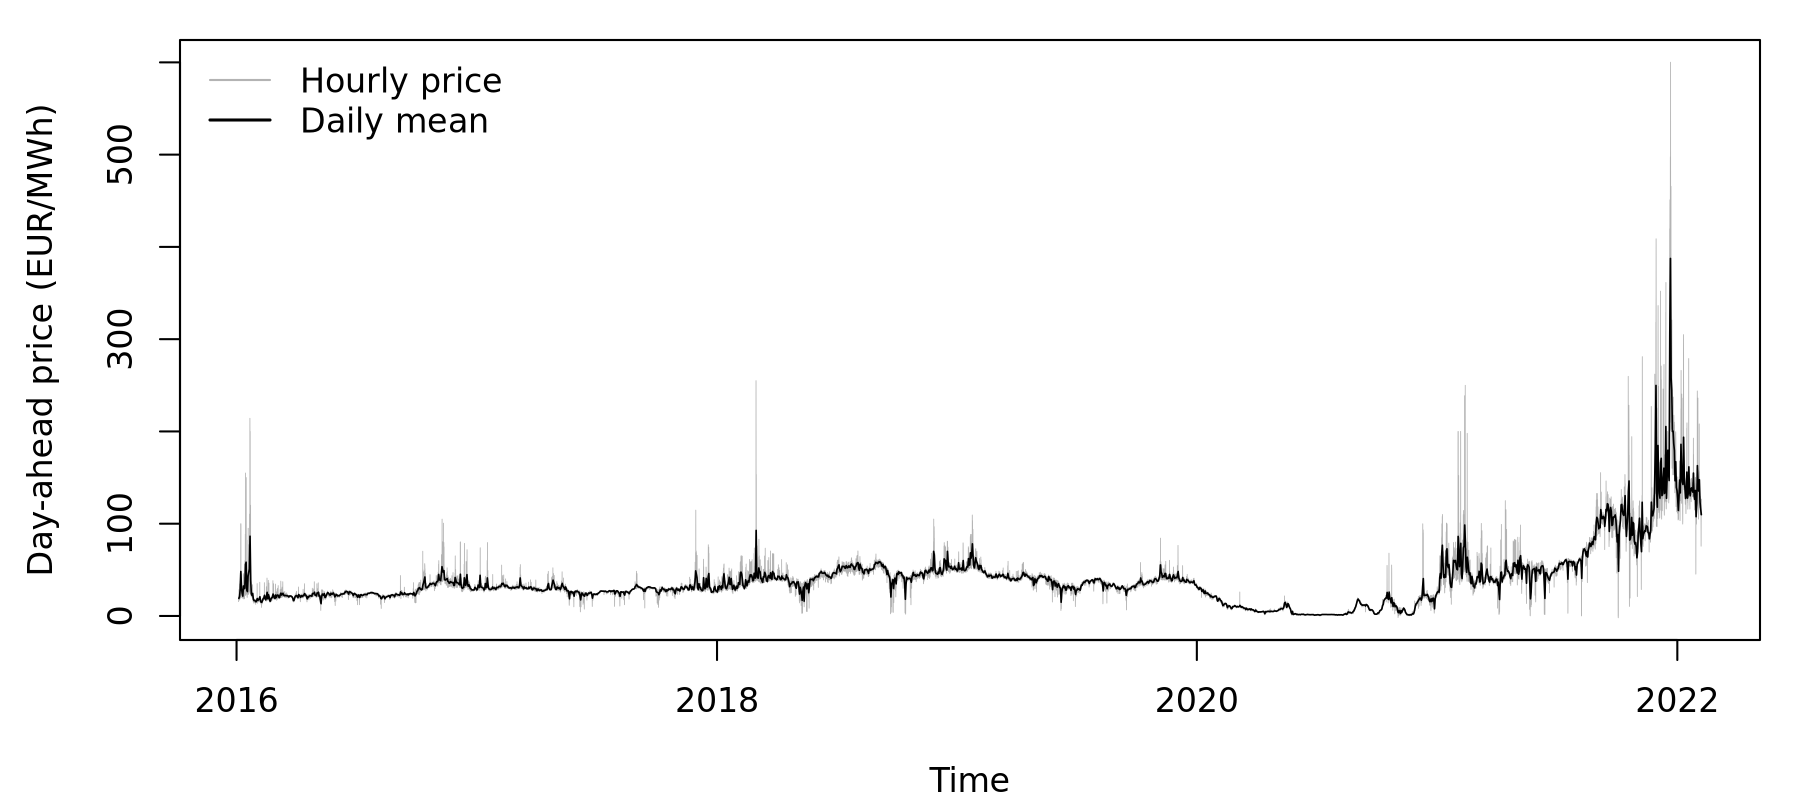
\includegraphics[width=\textwidth]{fig_price_time.png}
\end{column}
\end{columns}
\end{frame}

%------------------------------------------------------------
\begin{frame}{Data}
\begin{itemize}
\item My master thesis data: Nord Pool prices and consumption, NVE reservoir fill
\item Hourly, \cleanStart{} to \cleanEnd{}: \textbf{$n = \nClean$ hours}
\item Price in \eur{}, \nNonPos{} hours $\le 0$, max \maxPrice{}
\end{itemize}
\vspace{0.5em}
\textbf{Preparation}
\begin{itemize}
\item \nMissingPrice{} forward-filled prices removed ($\pctRemoved$\% in total)
\item Weekly reservoir value given to every hour of its ISO week
\item Factors from local time; reference: hour 00, January, Monday, 2016
\end{itemize}
\end{frame}

%------------------------------------------------------------
\begin{frame}{Method: Gaussian GLM}
\begin{itemize}
\item Price is continuous and can be zero or negative\\
$\Rightarrow$ not Poisson, binomial or Gamma; \textbf{normal} distribution
\item Identity link = multiple linear regression, coefficients in \eur
\end{itemize}
\begin{align*}
y_i = \bs{x}_i^T\bs{\beta} + e_i, \qquad e_i \sim N(0,\sigma^2)
\end{align*}
\vspace{-1em}
\begin{center}
\texttt{glm(price \textasciitilde{} hour + month + weekday + year + cons + reservoir,}\\
\texttt{family = gaussian)}
\end{center}
\begin{itemize}
\item Compare: drop-one $F$-test, AIC/BIC, $R^2$; VIF; residuals and ACF
\item GAM (\texttt{mgcv}) if curves show up
\end{itemize}
\end{frame}

%------------------------------------------------------------
\begin{frame}{Key results}
\begin{columns}[T]
\begin{column}{0.64\textwidth}
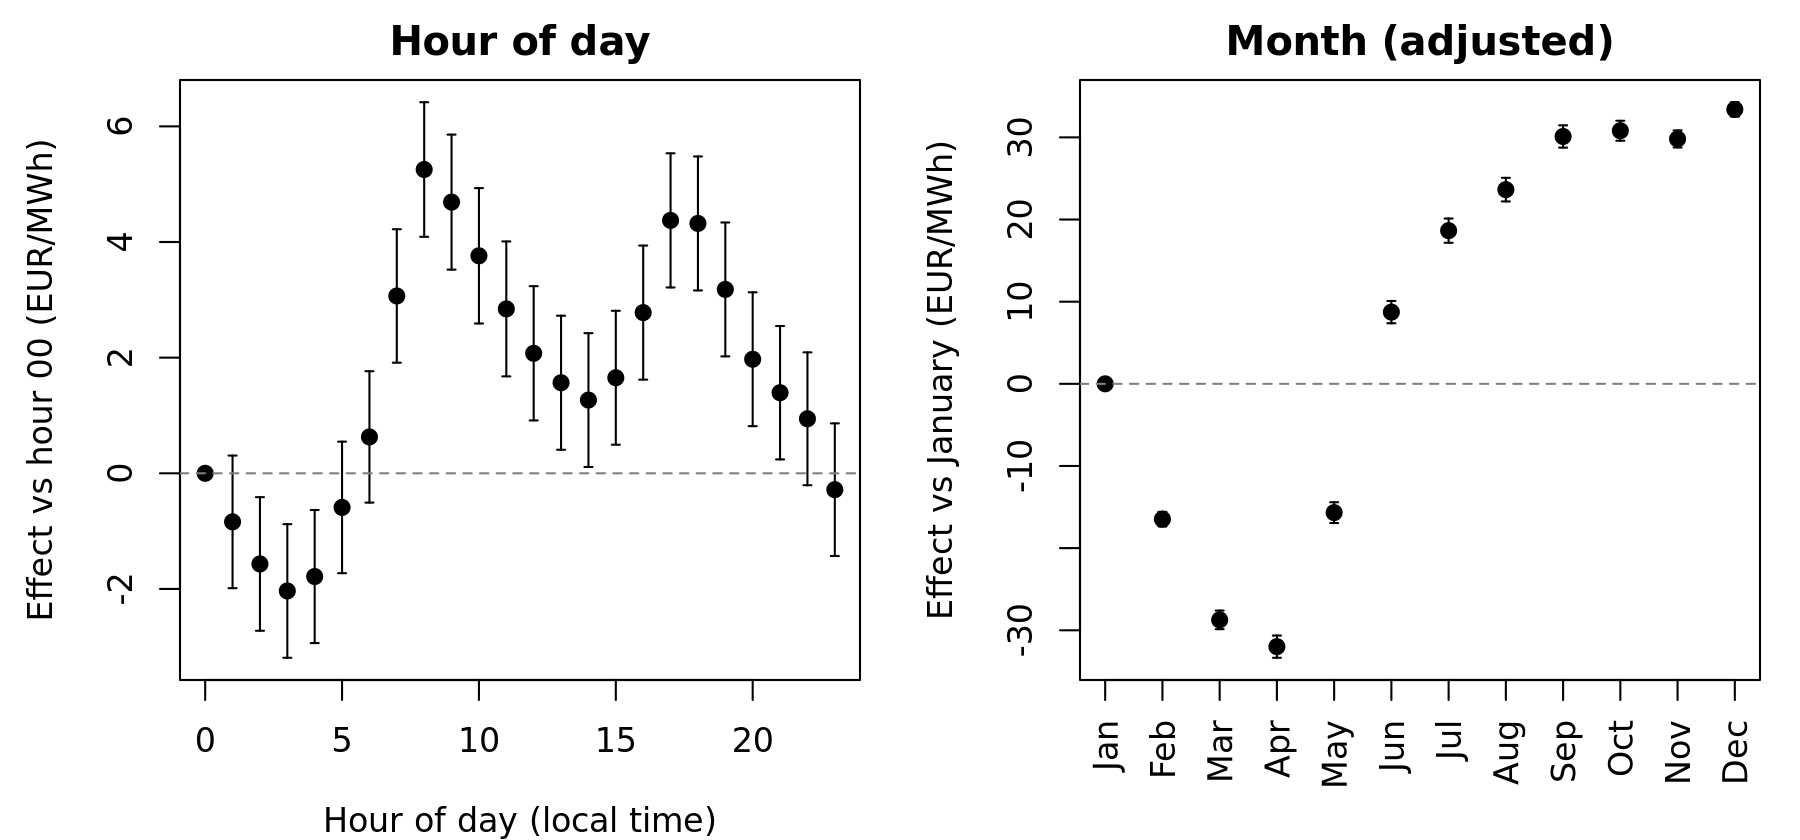
\includegraphics[width=\textwidth]{fig_effects.png}
\end{column}
\begin{column}{0.36\textwidth}
\small
\begin{itemize}
\item $R^2 = \rTwo$, $\hat\sigma = \rse$ \eur
\item Hour $\hMorning$: $+\bHourMorning$ vs midnight
\item Sunday: $\bSun$ vs Monday
\item 2021: $+\bYtwentyone$, 2022: $+\bYtwentytwo$ vs 2016
\item \textbf{Reservoir +10 points: $\bResTen$}
\item Consumption +1 GWh/h: $+\bCons$
\end{itemize}
\end{column}
\end{columns}
\end{frame}

%------------------------------------------------------------
\begin{frame}{Which predictors matter most?}
\centering
Loss when one term is removed from the full model\\[0.8em]
\begin{tabular}{lrr}
\toprule
Term removed & $\Delta R^2$ (\%-points) & $\Delta$AIC \\
\midrule
Year & \dRtwoYear & \dAICYear \\
Month & \dRtwoMonth & \dAICMonth \\
Reservoir & \dRtwoReservoir & \dAICReservoir \\
Hour & \dRtwoHour & \dAICHour \\
Weekday & \dRtwoWeekday & \dAICWeekday \\
Consumption & \dRtwoConsumption & \dAICConsumption \\
\bottomrule
\end{tabular}\\[1em]
\raggedright
\begin{itemize}
\item All $p < 0.001$ with $n = \nClean$: look at effect sizes
\item Collinearity: month explains \auxResMonth\% of reservoir, \auxConsMonth\% of consumption
\end{itemize}
\end{frame}

%------------------------------------------------------------
\begin{frame}{Model fit and diagnostics}
\begin{columns}[T]
\begin{column}{0.55\textwidth}
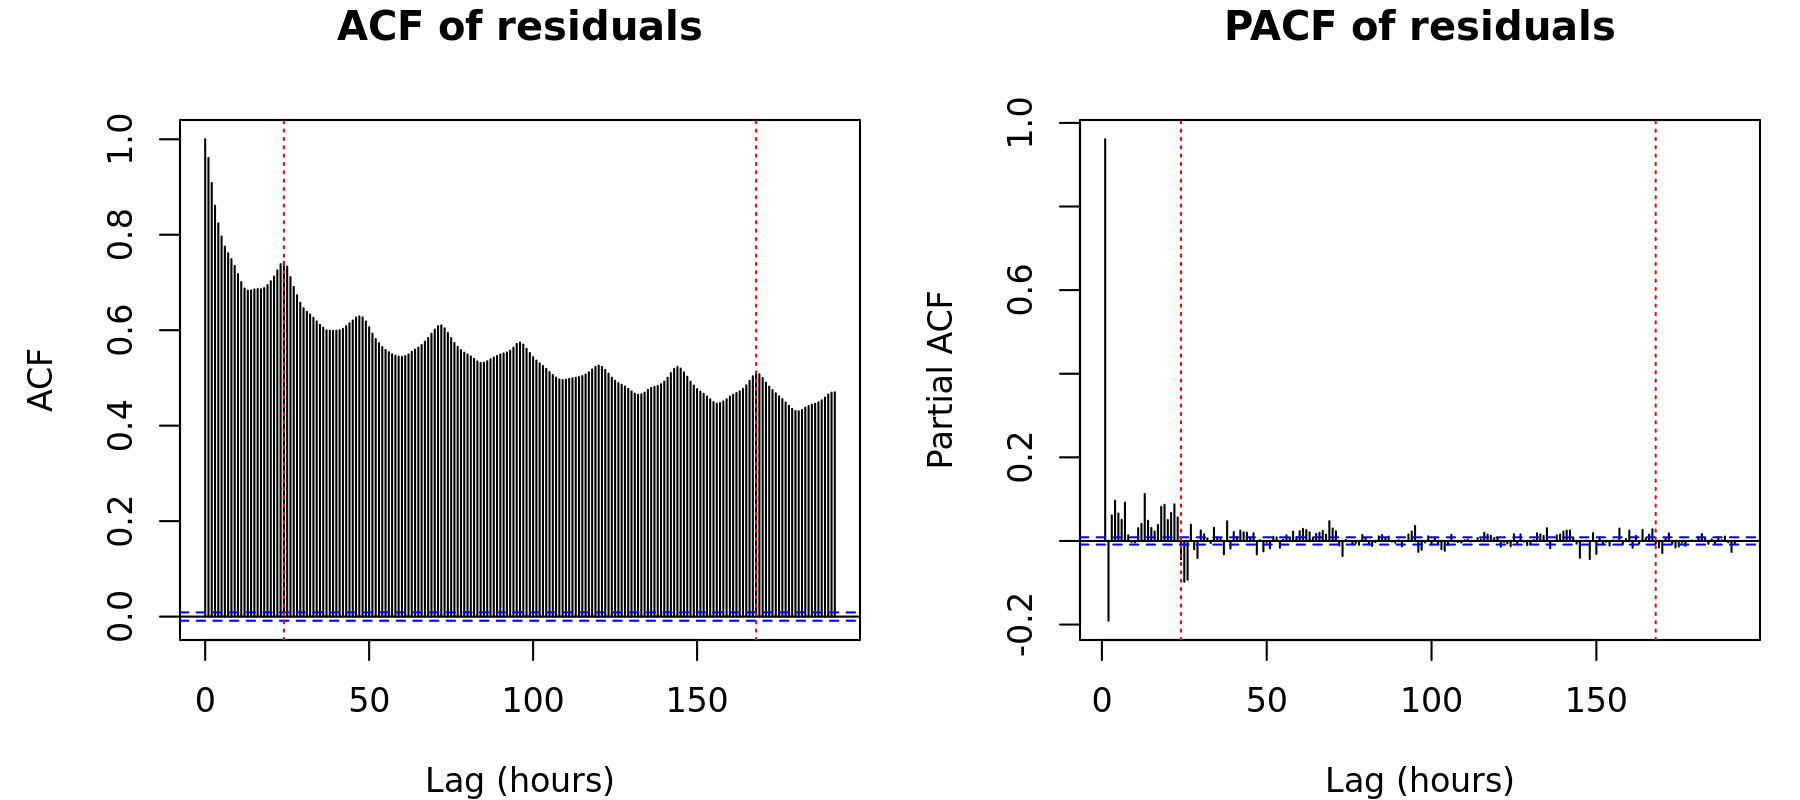
\includegraphics[width=\textwidth]{fig_acf.png}
\end{column}
\begin{column}{0.45\textwidth}
\small
\begin{itemize}
\item Lag-1 autocorrelation \acfOne, Durbin-Watson \dw
\item Variance grows with price, heavy upper tail (2021/22)
\item HAC SEs \hacRatioMin{} to \hacRatioMax{} times larger
\item Reservoir: still clear
\item \textbf{Consumption: $p = \pHacCons$}
\end{itemize}
\end{column}
\end{columns}
\end{frame}

%------------------------------------------------------------
\begin{frame}{GAM: non-linear effects}
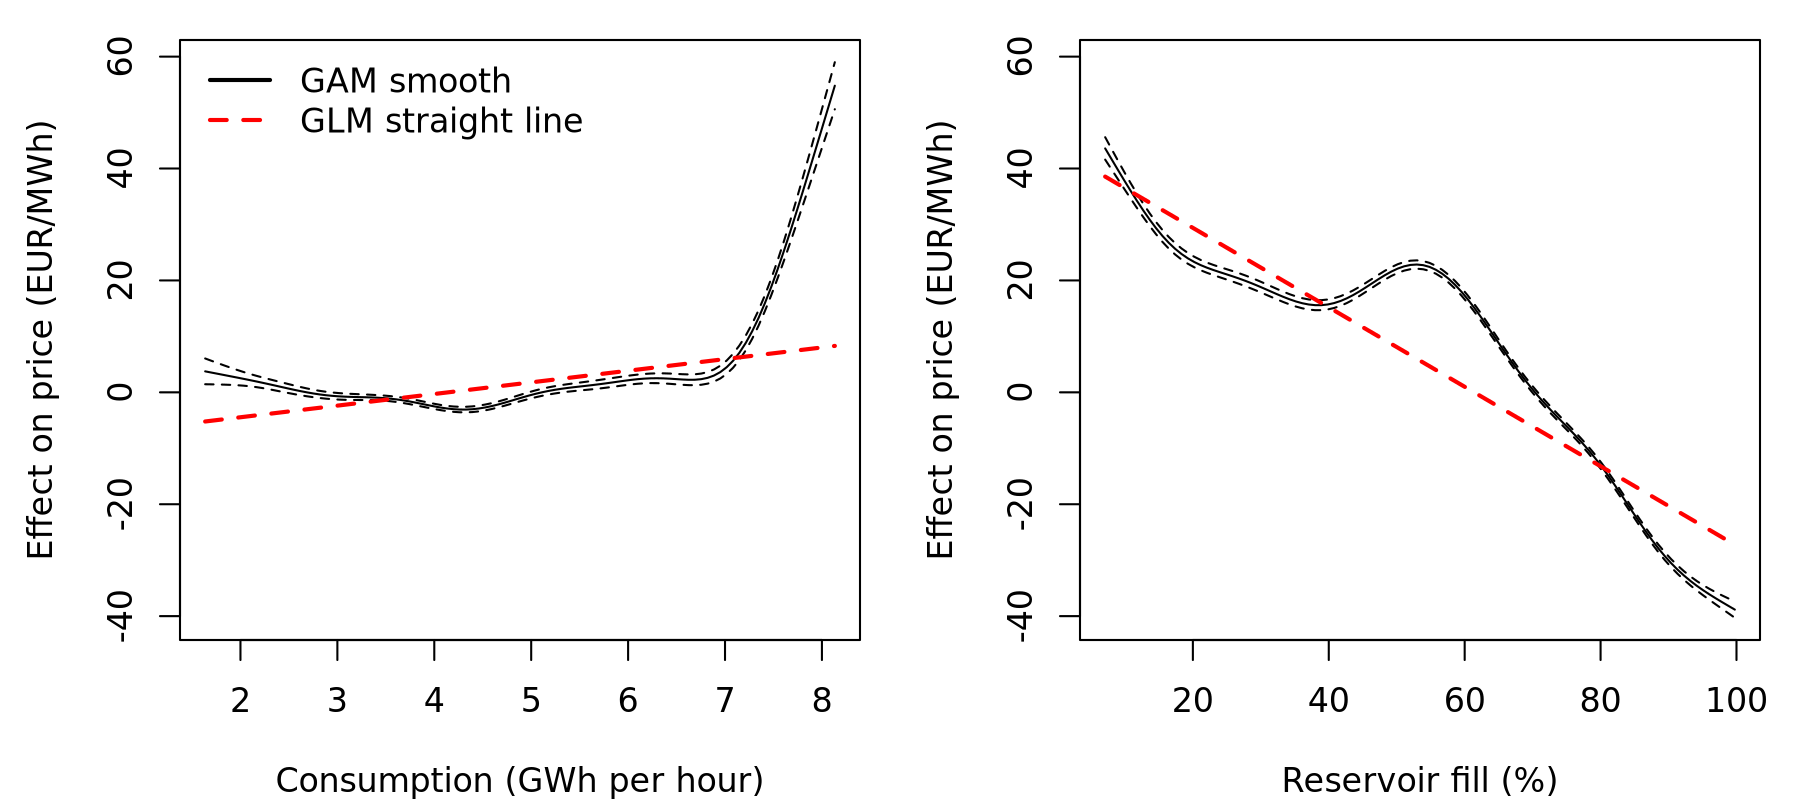
\includegraphics[width=0.8\textwidth]{fig_gam.png}
\begin{itemize}
\item Price jumps above 7 GWh/h; reservoir effect strongest at the ends
\item AIC $-\dAICGam$, $R^2$ \rTwo{} $\to$ \rTwoGam; same ranking of predictors
\end{itemize}
\end{frame}

%------------------------------------------------------------
\begin{frame}{In plain words, and limitations}
\textbf{In plain words}
\begin{itemize}
\item The year matters most: 2021/22 prices came from outside factors
\item Fuller reservoirs, cheaper power: about \bResTenAbs{} \eur{} per 10 points
\item Cheapest at night, most expensive around \hourMaxAt{} in the morning
\item Usage adds little, except in extreme cold hours
\end{itemize}
\textbf{Limitations}
\begin{itemize}
\item Strong autocorrelation: usual $p$-values too optimistic
\item Non-constant variance, crisis outliers
\item Year factor describes, does not explain
\end{itemize}
\end{frame}

%------------------------------------------------------------
\begin{frame}{Conclusion}
\begin{itemize}
\item Gaussian GLM explains $R^2 = \rTwo$; year $\gg$ month $>$ reservoir $>$ consumption
\item Reservoir effect robust to autocorrelation, consumption effect not; GAM: better fit, same conclusions
\end{itemize}
\end{frame}

\begin{frame}[shrink=20]{Sources}
\nocite{dobson2008glm, nordpool, nve, R, mgcvREML, sandwich, car, lmtest}
\scriptsize
\printbibliography[heading=none]
\end{frame}

\end{document}
